% !TEX encoding = UTF-8 Unicode
%%%%%%%%%%%%%%%%%%%%%%%%%%%%%%%%%%%%%%%%%
% Beamer Presentation
% LaTeX Template
% Version 1.0 (10/11/12)
%
% This template has been downloaded from:
% http://www.LaTeXTemplates.com
%
% License:
% CC BY-NC-SA 3.0 (http://creativecommons.org/licenses/by-nc-sa/3.0/)
%
%%%%%%%%%%%%%%%%%%%%%%%%%%%%%%%%%%%%%%%%%

%----------------------------------------------------------------------------------------
%	PACKAGES AND THEMES
%----------------------------------------------------------------------------------------

\documentclass{beamer}

\mode<presentation> {

% The Beamer class comes with a number of default slide themes
% which change the colors and layouts of slides. Below this is a list
% of all the themes, uncomment each in turn to see what they look like.

%\usetheme{default}
%\usetheme{AnnArbor}
%\usetheme{Antibes}
%\usetheme{Bergen}
%\usetheme{Berkeley}
%\usetheme{Berlin}
%\usetheme{Boadilla}
%\usetheme{CambridgeUS}
%\usetheme{Copenhagen}
%\usetheme{Darmstadt}
%\usetheme{Dresden}
%\usetheme{Frankfurt}
%\usetheme{Goettingen}
%\usetheme{Hannover}
%\usetheme{Ilmenau}
%\usetheme{JuanLesPins}
%\usetheme{Luebeck}
%\usetheme{Madrid}
%\usetheme{Malmoe}
%\usetheme{Marburg}
%\usetheme{Montpellier}
%\usetheme{PaloAlto}
%\usetheme{Pittsburgh}
%\usetheme{Rochester}
\usetheme{Singapore}
%\usetheme{Szeged}
%\usetheme{Warsaw}

% As well as themes, the Beamer class has a number of color themes
% for any slide theme. Uncomment each of these in turn to see how it
% changes the colors of your current slide theme.

%\usecolortheme{albatross}
%\usecolortheme{beaver}
%\usecolortheme{beetle}
%\usecolortheme{crane}
%\usecolortheme{dolphin}
%\usecolortheme{dove}
%\usecolortheme{fly}
%\usecolortheme{lily}
%\usecolortheme{orchid}
%\usecolortheme{rose}
%\usecolortheme{seagull}
%\usecolortheme{seahorse}
%\usecolortheme{whale}
%\usecolortheme{wolverine}

%\setbeamertemplate{footline} % To remove the footer line in all slides uncomment this line
%\setbeamertemplate{footline}[page number] % To replace the footer line in all slides with a simple slide count uncomment this line

%\setbeamertemplate{navigation symbols}{} % To remove the navigation symbols from the bottom of all slides uncomment this line
}

\usepackage{graphicx} % Allows including images
\usepackage{booktabs} % Allows the use of \toprule, \midrule and \bottomrule in tables
\usepackage{xeCJK}
\setCJKmainfont{SourceHanSerif-Regular}
\usepackage{color}
\usepackage{listings}
\lstset{numbers=left}
\usepackage{tikz}


%----------------------------------------------------------------------------------------
%	TITLE PAGE
%----------------------------------------------------------------------------------------

\title[专业网站建设]{专业网站建设} % The short title appears at the bottom of every slide, the full title is only on the title page
\subtitle{概述}
\author{} % Your name
\institute[计算机科学与技术学院] % Your institution as it will appear on the bottom of every slide, may be shorthand to save space
{
贵州大学 \\ % Your institution for the title page
\medskip
\textit{hnzhang1@gzu.edu.cn} % Your email address
}
\date{\today} % Date, can be changed to a custom date

\begin{document}

\begin{frame}
\titlepage % Print the title page as the first slide
\end{frame}
\begin{frame}{Overview}
\tableofcontents
\end{frame}
\section{网站概述}
\subsection{网站和网络}
\begin{frame}{网站和网络}
互联网的起源于1969 美国的ARPANET,
中国于1994年接入国际互联网。

大致的发展历程如下:web1.0(门户网站和搜索);web2.0(2006年左右,SNS和BLOG);web3.0(目前还没有共识)
\end{frame}
\subsection{主流开发语言}
\begin{frame}{github repository of web development language (2019.3.5)}
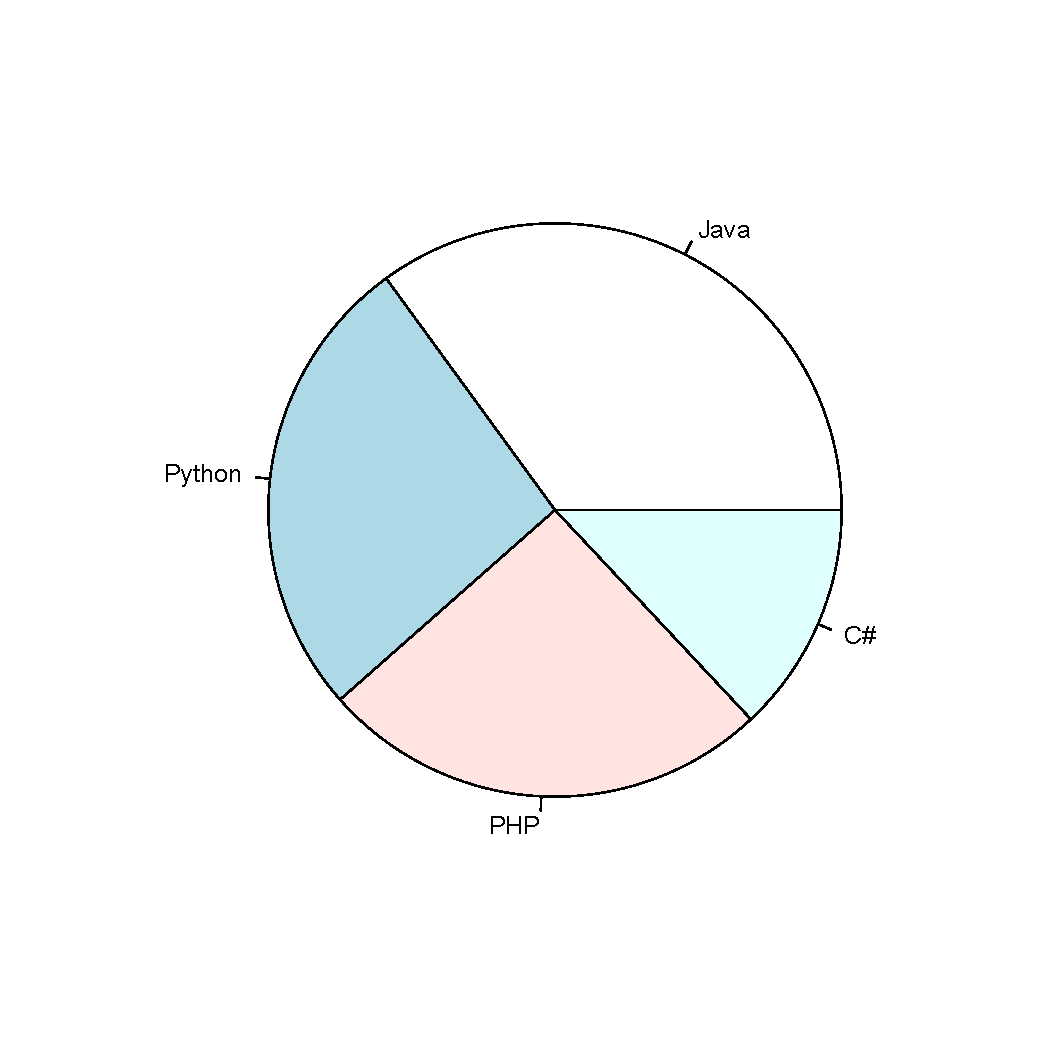
\includegraphics[height=1\textheight]{webLanguage.pdf}
\end{frame}
\subsection{python framework}
\begin{frame}{github repository of python web framworks (2018.12.24)}
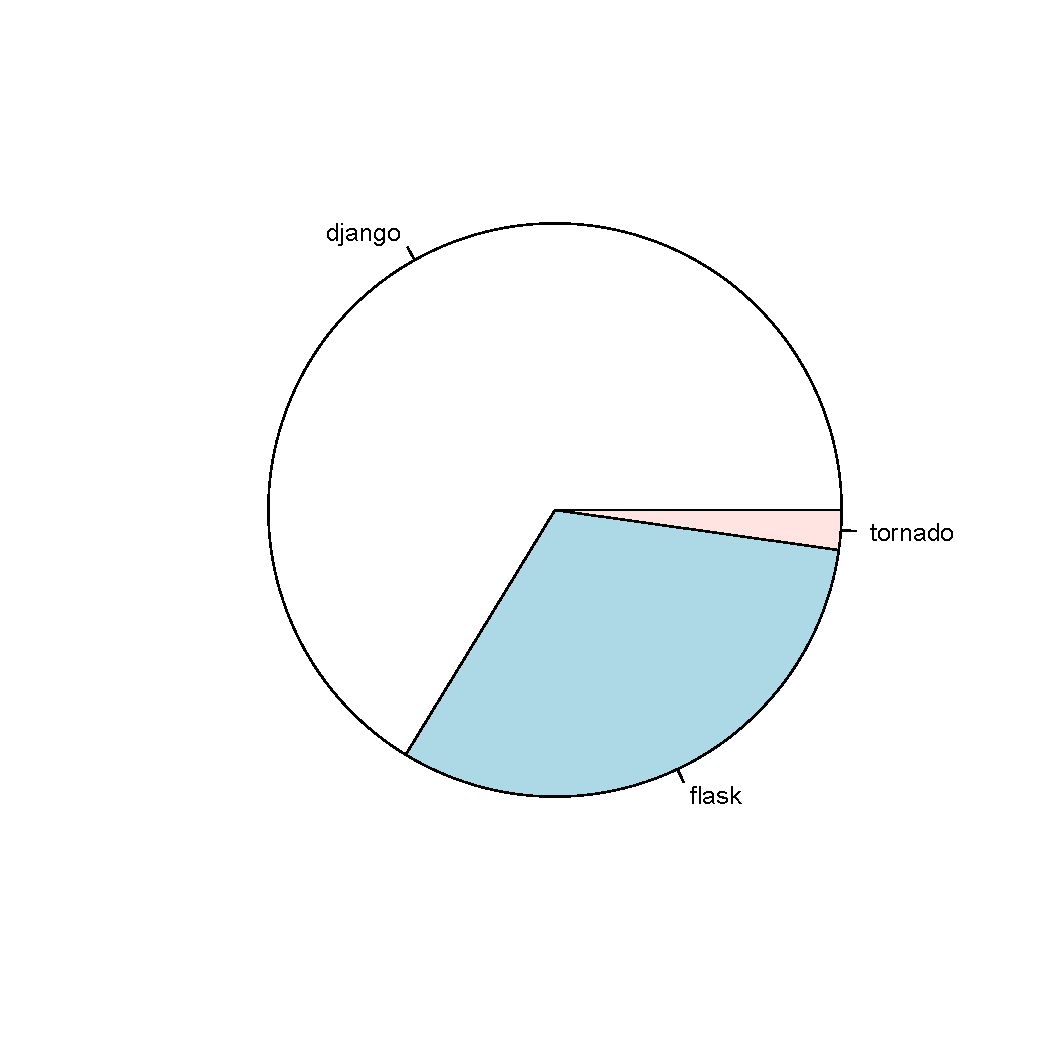
\includegraphics[height=1\textheight]{django-introduce-1.pdf}
\end{frame}
\section{课程概述}
\subsection{课程定位}
\begin{frame}{课程定位}
\begin{enumerate}
\item 了解网站建设的流程
\item 掌握python语言
\item 掌握简单动态网站的开发
\end{enumerate}

\end{frame}
\subsection{课程所涉及到的内容}
\begin{frame}{课程所涉及到的内容}
\begin{enumerate}
\item HTML相关知识
\item python语言
\item django框架
\end{enumerate}

\end{frame}
\subsection{考核方式}
\begin{frame}{考核方式}
\begin{description}
\item[ 15\% ] 平时考勤(点名+作业+实验报告)
\item[ 35\% ] python编程测试(5道编程题) 
\item[ 50\% ] 博客系统项目答辩
\end{description}

\end{frame}
\subsection{ppt下载地址}
\begin{frame}{ppt下载地址}
\url{https://github.com/gmsft/ppt/tree/master/django}
\end{frame}
\end{document} 

